\chapter{Psi}
%TODO Die Introduction fängt gut an, aber MicroPsi fällt mir zu sehr vom Himmel. Du solltest in der Introduction wirklich nur motivierend bleiben, warum will man so was wie MicroPsi haben, warum braucht man Simulationsumgebungen, keine Details zur MicroPsi-Implementierung oder Minecraft. Das kommt erst im Kapitel Foundations (dort kannst du den Text wahrscheinlich ziemlich so bringen, wie er in der Motivation steht)!

A widely accepted definition of the field of AI is that it is the study and design of intelligent agents, where an intelligent agent is a system that perceives its environment and takes actions that maximise its chances of success. %TODO find original sources

It took many years for AI research to evolve from the early ideas of thinking machines over Deep Blue, the computer that could beat mankind's best chess players to Watson, the AI that beats the champions of Jeopardy, the game show, that is about asking the appropriate question to a given answer. There exist many applications for AI~. Self-driving cars and online-shopping recommendation systems to name a few.

These examples have one thing in common. They are applications of technology that serves an immediate, or at least foreseeable purpose. For AI in scenarios of this kind, the term applied AI (or weak AI) has been coined.

Strong AI, in contrast, is about researching the nature of intelligence itself. An actual (hypothetical) implementation of a Strong AI translates to building a machine, that is capable of acting like a human being --- not just in a defined problem fields, but in all of them.

Cognitive AI, in particular, can be thought of as architectures that implement findings and theories in the fields cognitive science and psychology, as well as the neuro-sciences, for the sake of proving, if the theories hold against what they promise. 

%... Examples for cognitive architectures are ...

Many cognitive architectures share characteristics with or directly implement artificial neural node nets.

%... Approaches to cognitive AI ...
%... neural node nets ...
%... related work ...

\section{Psi Theory}
The Psi theory in its foundations was described by german psychologist Dietrich Dörner in his books ``Bauplan für eine Seele'' and ``Die Mechanik des Seelenwagens'' from 1998 and 2002. Dörners holistic approach goes beyond classic problem solving but developes a unified model for cognition that implements motivation and emotions.
It's main ideas are, that it thinks of cognition as a graph-like structure (e.g. node-net) of relationships that strives to maintain homeostatic balance.\cite{Bach:2009:PSI:1611304}

Basic components of the theory are Representation, Memory, Perception, Drives, Cognitive modulation and emotion, Motivation, Learning and Problem solving as well as Language and consciousness. %(wikipedia)

%TODO describe it myself
``The PSI theory is a theory of human action regulation by psychologist Dietrich Doerner. It is an attempt to create a body-mind link for virtual agents. It aims at the integration of cognitive processes, emotions and motivation. This theory is unusual in cognitive psychology in that emotions are not explicitly defined but emerge from modulation of perception, action-selection, planning and memory access. Emotions become apparent when the agents interact with the environment and display expressive behavior, resulting in a configuration that resembles emotional episodes in biological agents. The agents react to the environment by forming memories, expectations and immediate evaluations. This short presentation is a good overview.

PSI agents possess a number of modulators and built-in motivators that lie within a range of intensities. These parameters combined to produce complex behaviour that can be interpreted as being emotional. Additionally, by regulating these parameters, the agent is able to adapt itself to the different circumstances in the environment. This theory has been applied to different virtual agent simulations in different types of environments and has proven to be a promising theory for creation of biologically plausible agents.'' %(wikipedia)


%... Basics of Psi Theorie of Dörner ...

Joscha Bach adapted that theory to bring it in a contemporary from with slight modifications.

%... explanation of Joschas Dissertation ...

%\section{Summary}
Even though building a conscious machine that thinks and acts like we do is still mehre science-fiction, it is this kind of foundational research, that leads no new ways of thinking of the world, that give us our most import leaps.

%... still a lot to do in AI ...

This project is fundamentally about combining existing technologies. In particular, the two most important ones are MicroPsi 2, the most ambitious framework aiming to implement the ideas of the Psi theory, and Minecraft, the super-popular sandbox-videogame.

To understand how and why they were chosen, a brief history of their creation as well as explanations of their basic ideas and relevant insights to their architecture are what this chapter is about.

    \section{Psi Implementations}
Psi has been implemented by different groups at different times. The first implementations are by Dörner and his associates themselves~(see figure \ref{psi_screen}). They used Pascal and developed it for windows environments. This implementation can still be downloaded and runs on Windows 7 installations, for example.

\begin{figure}[h]
  \centering
    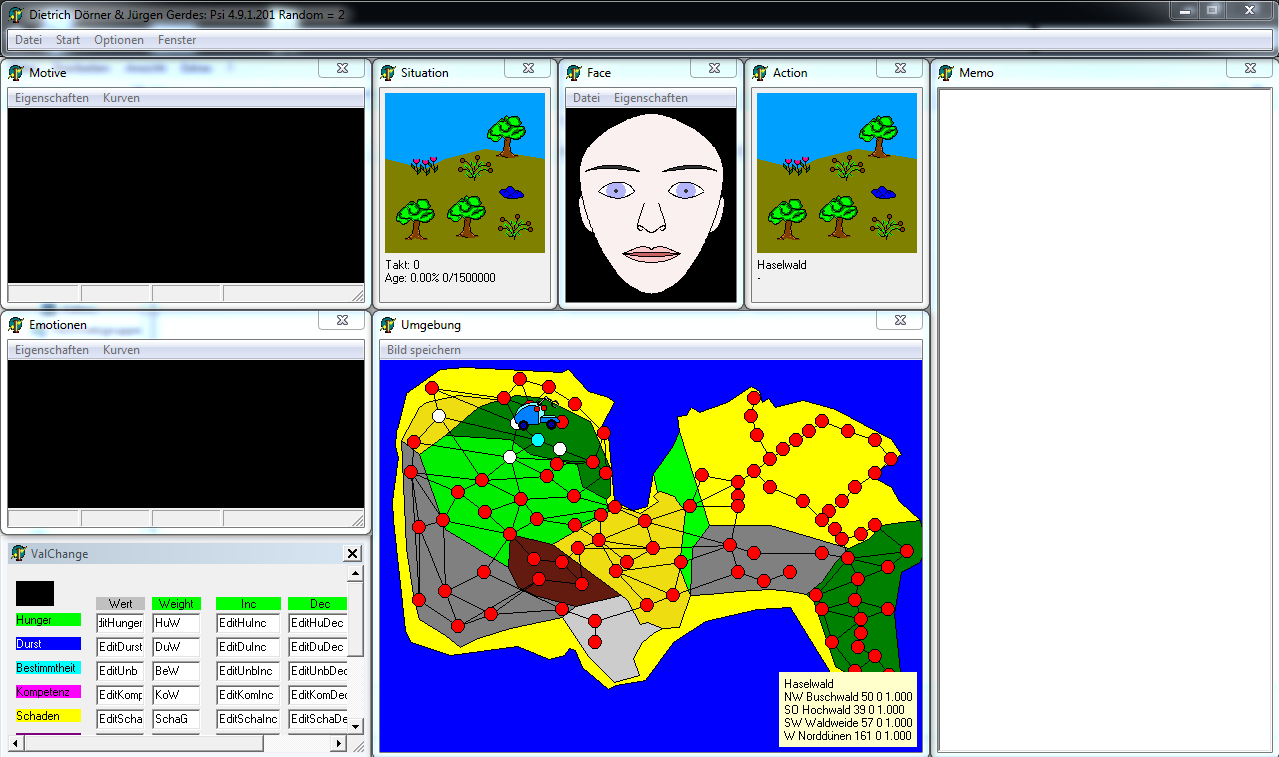
\includegraphics[width=10cm]{graphics/psi_screen1}
  \caption{Dörner's Pascal Psi Implementation}
  \label{psi_screen}
\end{figure}

The work on Dörner's team's implementation has not been continued, so Joscha Bach and his associates built new implementations of Psi.

From 2003 to 2009 they built an implementation in Java as a set of plugins for the Eclipse IDE called MicroPsi. It included of a graphical editor and a 3D simulation-environment. Aiming at better understandability and to maintain platform independence, MicroPsi has been built ground up again in 2012 --- using more lightweight Python code. What is remarkable about the new implementation called MicroPsi 2 (in the following MicroPsi), is that the simulation is deployed as a web application and the graphical interface is completely rendered inside a web browser --- using state-of-the-art internet- and webapplication-technologies. It is based upon HTML as well as Javascript and the communication in between the browser and the simulation is managed via JSON remote procedure calls. Many GUI components of Twitter's Bootstrap library as well as the JavaScript graphics library PaperJS are used.~\cite{conf/agi/Bach12}

According to the concepts of the Psi Theory, MicroPsi simulates agents as neuro-symbolic spreading activation networks. Agents can be placed and researched in simulation environments or physically embodied as robots.~\cite{conf/agi/Bach12}
        
Even though there have been more complex simulation environments (e.g. 3D-worlds) for previous implementations of Psi-architectures, the relatively new version of MicroPsi has only two fairly simple ones: a 2D-Island and a map of the public transportation system of Berlin~(see figure~\ref{mp2_berlin}). Instead of building another 3D-world, with this project we set out for something more experimental.

\begin{figure}[h]
  \centering
    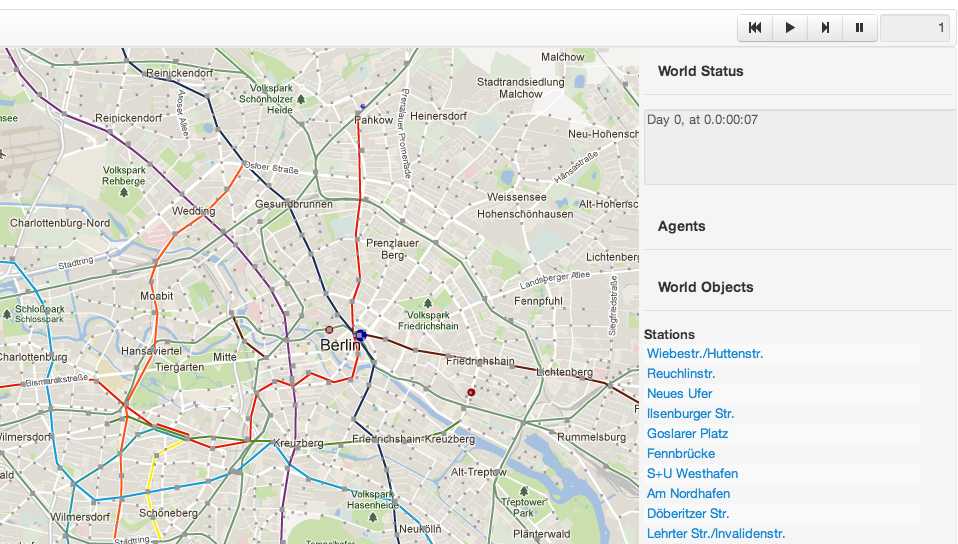
\includegraphics[width=10cm]{graphics/mp2_berlin}
  \caption{MicroPsi simulation environment Berlin}
  \label{mp2_berlin}
\end{figure}

        \section{MicroPsi 2 Module Overview}
MicroPsi's modular structure is fairly easy to understand~(see figure ~\ref{micropsi2_modules}). At first, one can differentiate between the server component (or the web-interface) and the actual simulation code (called "core").

In a minimal setup MicroPsi runs three threads. One thread for the web server, one for the world simulation and one for every world-adapter (or agent). If more then one agent or more than one world are launched, they are instantiated as additional threads.

Furthermore, the core consists of a runtime component, a user and a configuration manager. The runtime works independently of the server and can also by deployed for command line interaction or other GUIs. It manages the simulations worlds as well as the agents (node net embodiments) and the world-adapters.~\cite{conf/agi/Bach12}
\\          
          
\begin{figure}[h]
  \centering
    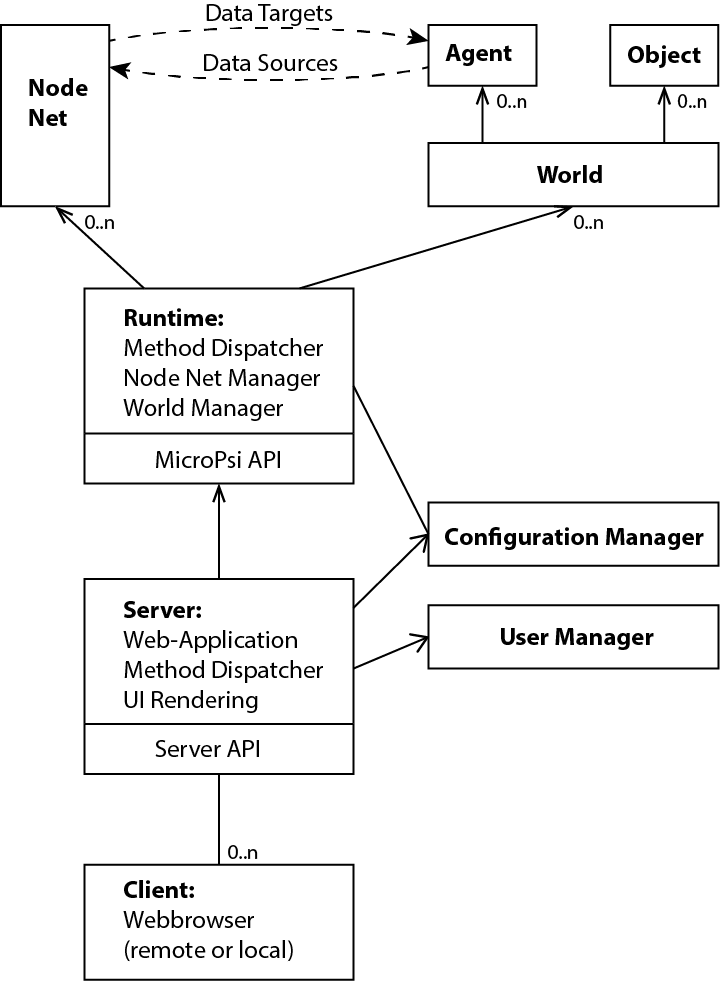
\includegraphics[width=10cm]{graphics/micropsi2_uml}
  \caption{The MicroPsi 2 architecture~\cite{conf/agi/Bach12}}
  \label{micropsi2_modules}
\end{figure}
            
        \paragraph{Agents}
MicroPsi defines agents as node nets or, to be more specific, hierarchical spreading activation networks. They are an "abstraction of the information processing provided by brains"~\cite{conf/agi/Bach12}. The assigned world-adapter provides data sources and data targets to manage the communication in between the node net and the simulation environment. They represent the agent's sensory input and motoric output. Sophisticated interconnection of those enables interaction with the environment.~\cite{conf/agi/Bach12}
       
        \paragraph{Worlds}
The simulations worlds are the environments in which we can study our agent's behaviour. Worlds need to provide a world adapter --- the interface in between a node net and the simulation. Data sources and data targets have to be defined carefully, to get a functional and meaningful experiment going. Node nets and environments may be updated asynchronously.~\cite{conf/agi/Bach12}

The kind of data the world adapter interfaces, is not specified any further, which gives developers the opportunity to experiment with classic simulation worlds as well as exotic applications (eg. stock data). At the time of the original development of the framework, the priorized application was building a framework for knowledge representation.~\cite{conf/agi/Bach12}
